\section{Analysis of experimental data}

We have verified that de-noising of background merged files significantly improves the track reconstruction efficiency.
It was shown that using AI assisted version of reconstruction software further improved the number of particles reconstructed for given reaction. 
The further checks experimental data collected with $45~nA$ incident beam energy was processed using de-noising software and then was processed with CLAS12 data reconstruction program. The same reaction $H(e,e^\prime\pi^+\pi^-)X$ was selected (for consistency) from experimental data and missing mass distributions were plotted for raw data, de-noised data reconstructed with conventional tracking algorithm and de-noised data reconstructed with AI assisted tracking algorithm.
The results are shown on Figure~\ref{denoise:exp_data}


\begin{figure}[!h]
\begin{center}
 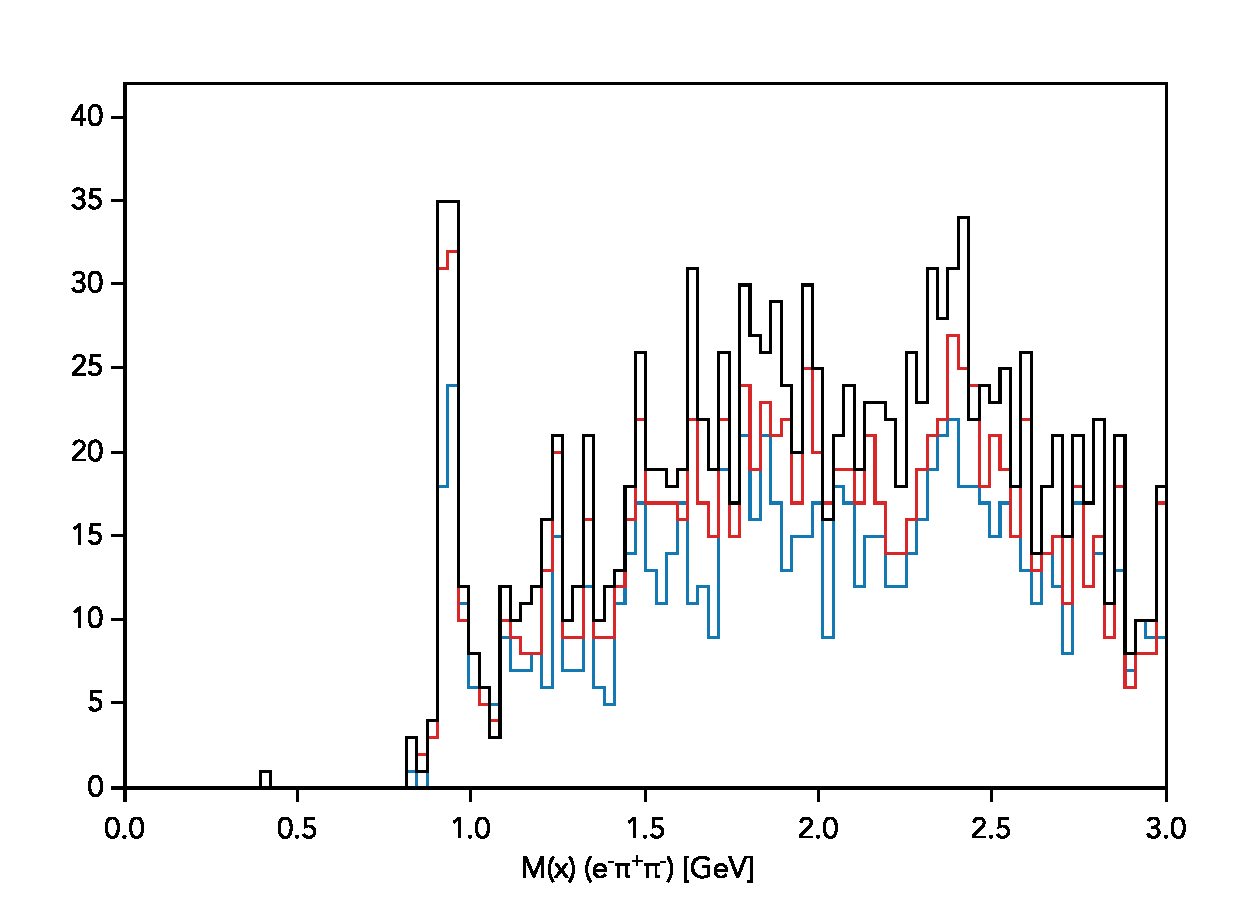
\includegraphics[width=3.1in]{images/figure_denoise_expdata.pdf}
\caption {Tracking efficiency as a function of luminosity (beam current) for positive (a) and negative particle (b).  The efficiency is shown for
conventional algorithm running on background merged files (diamonds), and on files with merged background then de-noised with AI (circles).}
 \label{denoise:exp_data}
 \end{center}
\end{figure}


\begin{table}[!h]
\begin{center}
\begin{tabular}{lccc}
Method & protons count & ratio &  MC ratio \\
\hline
Conventional & 41 & 1.00 & 1.00 \\
De-Noised & 59 & 1.43 & 1.37 \\
De-Noised with AI assisted & 70 & 1.71 &1.65 \\
\hline
\end{tabular}
\end{center}
\end{table}


